% -*-latex-*-
% Lecture for Computational Intelligence, Chapter 10

\documentclass[12pt]{beamer} % mathserif for normal math fonts.
\usefonttheme[onlymath]{serif}
\usepackage[utf8]{inputenc}
%\usepackage[swedish,english]{babel}
%\usepackage{amsmath,mathtools}
\usepackage{calc}
\usepackage{graphicx}
\usepackage{float}
\usepackage{color}

\usepackage[T1]{fontenc}

% The Chalmers theme:
\usetheme[titleflower=false]{chalmers} % titleflower = true or false
\title{Reasoning under Uncertainty Part~II}
\subtitle{Artificial Intelligence, 2015\\ TIN172/DIT410} % optional
\author[Olof Mogren]{Olof Mogren\\ \tiny{based on slides by\\ Poole, Mackworth\\ (Licensed under Creative Commons BY-NC-SA v4.0)}} % [short author (optional)]{many authors}
\institute{Chalmers University of Technology}
%\titlepageextra{Some conference} % Optional extra info, appears before date on title page
%\footer{\insertshortauthor\ Some conference} % optional, manually sets footer (default is short author)
\footer{Reasoning under Uncertainty - \insertshortauthor} % but it can of course be anything.
%\titlepagelogofile{../chalmersfigures/chalmers_textlogo} % File name to the file you want to include.
%\titlepagelogo{\tikz{\draw(0,0) circle (1);}} % or draw anything for a logo


\newcommand{\figdir}{../../figures/ch06}

\begin{document}


%\section{~} % Sections are shown at the bottom left. There is also links in many pdf-readers
\begin{frame}[plain]
 \titlepage
\end{frame}

\begin{frame}
\frametitle{Quick recap: Random Variables}
\begin{itemize}
\item Upper case: $X$.
\item Value is subject to chance.
\begin{itemize}
\item Values: lower case.
\item Could represent the outcome of an experiment.
\end{itemize}
\item A probability $\in [0,1]$ is associated to each value that $X$ can take.
\end{itemize}
\begin{center}
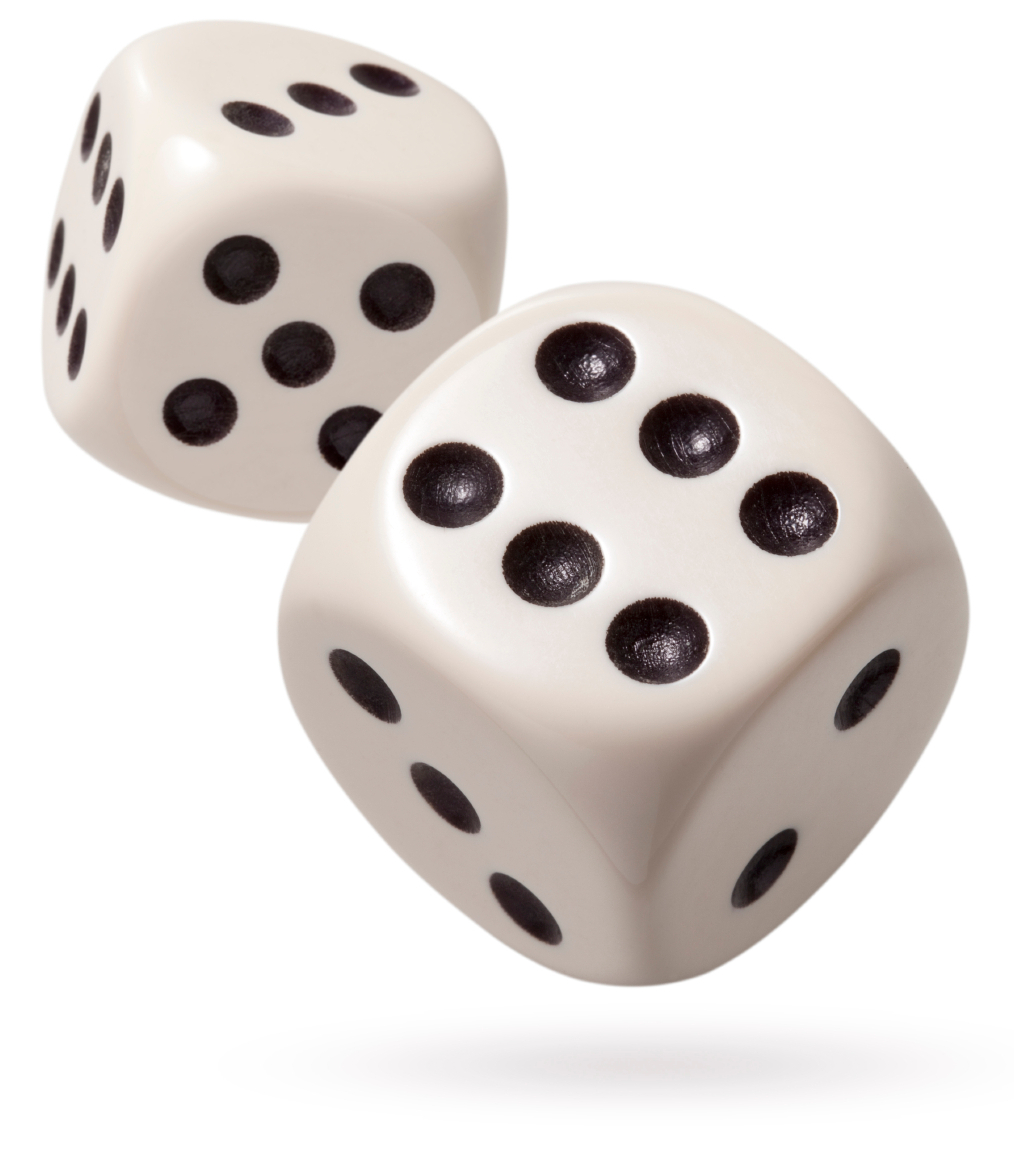
\includegraphics[width=0.3\columnwidth]{figures/uncert_fig_dice1.jpg}
\end{center}
\end{frame}


\begin{frame}
\frametitle{Quick recap: Probability Distributions}
\begin{columns}
    \begin{column}{0.6\textwidth}
\begin{itemize}
\item Describes the behaviour of a random variable.
\item $P(X)$ is the probability measure of $X$.
\item More than one variable:
\begin{itemize}
\item Joint: $P(X, Y, Z)$
\item Marginal: $P(X) = \sum_Y P(X,Y)$
\item Conditional: $P(X|Y) = \frac{P(X,Y)}{P(Y)}$
\end{itemize}
\end{itemize}
    \end{column}
    \begin{column}{0.4\textwidth}
\begin{center}

\includegraphics[width=\columnwidth]{figures/uncert_fig_tossingcoin.png}
\end{center}
    \end{column}
\end{columns}
\end{frame}


\begin{frame}
\frametitle{Example: Probability Distributions}
$X$ - The outcome of a coin toss
\begin{columns}
    \begin{column}{0.75\textwidth}
\begin{itemize}
\item This is called the \textbf{Binomial distribution}
\item $P(X=heads)$ - the probability that coin comes up heads
\item $P(X=tails) = 1-P(X=heads)$
\end{itemize}
    \end{column}
    \begin{column}{0.25\textwidth}
\begin{tabular}{|l|r|}
\hline
$X$ & $P(X)$\\
\hline
heads & 0.5\\
tails & 0.5\\
\hline
\end{tabular}\\

\begin{center}

\includegraphics[width=\columnwidth]{figures/uncert_fig_tossingcoin.png}
\end{center}
    \end{column}
\end{columns}
\end{frame}


\begin{frame}
\frametitle{Chain Rule for Probabilities}
\begin{align*} P(X, Y, Z) &=
P(X | Y, Z) P(Y, Z) 
\only<2> {\\ &= P(X | Y, Z) P(Y | Z) P(Z)} \end{align*}

\end{frame}


\begin{frame}
\frametitle{Conditional Independence}
\[ X \bot Y | Z \rightarrow P(X|Y,Z) = P(X|Z) \]
\end{frame}


\begin{frame}
\frametitle{Probability Distributions ctd.}
\begin{itemize}
\item Belief networks.
\begin{itemize}
\item Nodes: random variables.
\item Arcs: causal dependence
\item Network encodes independence.
\item Flow of influence.
\end{itemize}
\end{itemize}
\end{frame}


\begin{frame}
\frametitle{Example Belief Network}
\begin{center}
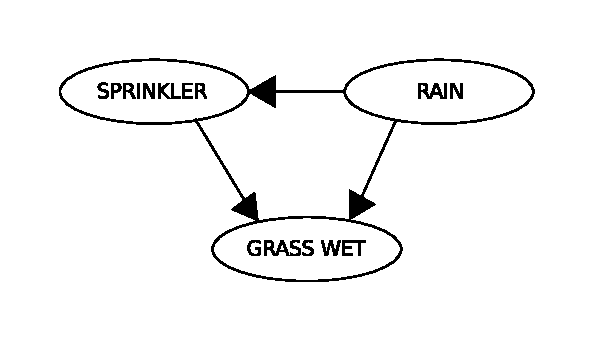
\includegraphics[width=0.8\textwidth]{figures/uncert_fig_bayes-net.pdf}
\end{center}
\end{frame}


\begin{frame}
\frametitle{Chain Rule for Bayesian Networks}
\begin{itemize}
\item Chain rule for Bayesian Networks:
\[ P(X_1, X2, X3, ..., X_n) = \prod_{i} P(X_i | parents(X_i)) \]
\item P factorizes over the network.
\end{itemize}
\end{frame}


\begin{frame}
\frametitle{Example Belief Network}
\begin{center}
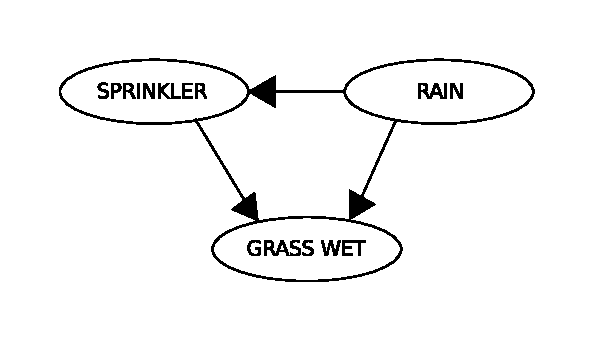
\includegraphics[width=0.6\textwidth]{figures/uncert_fig_bayes-net.pdf}
\end{center}
\begin{itemize}
\item Using the chain rule:
$ P(Grass, Sprinkler, Rain) = $\\
                              $P(Grass | Sprinkler, Rain)P(Sprinkler | Rain)P(Rain)$
                              \item A factorization of P.
                              \end{itemize}

                              \end{frame}


                              \begin{frame}
                              \frametitle{Querying Belief Networks}
                              \begin{itemize}
                              \item Query variable(s): $Q$
                                                        \item Observed evidence: $E_1=e_1, E_2=e_2, \dots, E_n=e_n$
                                                        \item How do you calculate $P(Q|e)$?
                                                        \end{itemize}

                                                        \end{frame}


                                                        \begin{frame}
                                                        \frametitle{Inference in Belief Networks}
                                                        \begin{enumerate}
                                                        \item Set observed evidence: $E_1=e_1, E_2=e_2, \dots, E_n=e_n$
                                                        \item Marginalize out non-query variables $W$ .
                                                        \item $P(Q|e) \propto \sum_W P(Q, W, E=e)$
                                                        \item Renormalize.
                                                        \end{enumerate}

                                                        \end{frame}


                                                        \begin{frame}
                                                        \frametitle{Renormalization}
                                                        \begin{itemize}
                                                        \item $\tilde{P}(X)$ - an unnormalized probability measure.
                                                        \item $P(X) = \frac{\tilde{P}(X)}{\sum_X \tilde{P}(X)}$ - renormalized probability distribution over X.
                                                        \item The denominator, $\sum_X \tilde{P}(X)$ is merely a constant.
                                                        \end{itemize}

                                                        \end{frame}


                                                        \begin{frame}
                                                        \frametitle{Example Belief Network}

                                                        \begin{center}
                                                        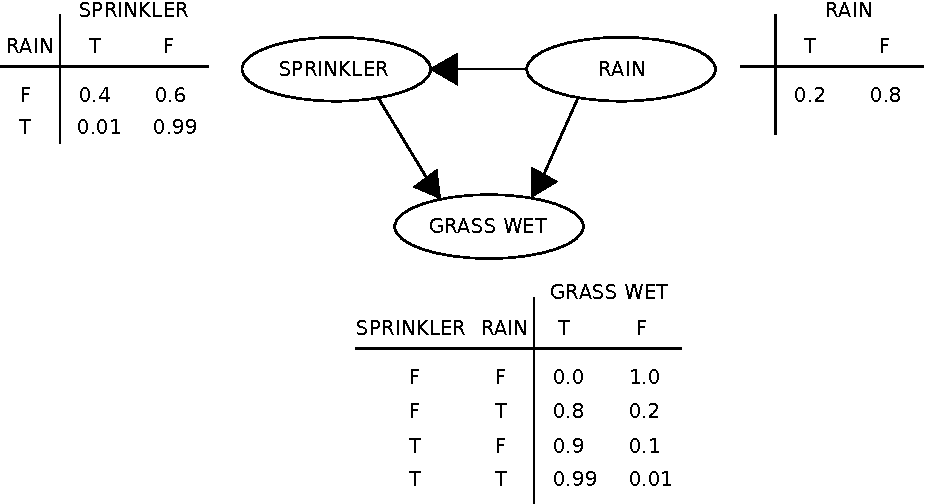
\includegraphics[width=0.9\textwidth]{figures/uncert_fig_bayes-net-w-cpds.pdf}
                                                        \end{center}

                                                        \end{frame}


                                                        \begin{frame}
                                                        \frametitle{Factors in general}
Function: $f(X_1,\ldots,X_j)$.

Assignments:
\begin{itemize}
\item
$f(X_1=x_1,X_2,\ldots,X_j)$,
  is a factor on
  $X_2,\ldots,X_j$.
  \item
  $f(X_1=x_1,X_2=x_2,\ldots,X_j=x_j)$
  \end{itemize}
  %The former is also written as $f(X_1,X_2,\ldots,X_j)_{X_1=v_1}$, etc.
  \end{frame}

  \begin{frame}
  \frametitle{Example factors}
  $r(X,Y,Z)$:\begin{tabular}{|lll|r|}
  \hline
  $X$ & $Y$ &$Z$ & val\\\hline
  t & t & t & 0.1\\
    t & t & f & 0.9\\
    t & f & t & 0.2\\
    t & f & f & 0.8\\
    f & t & t & 0.4\\
    f & t & f & 0.6\\
    f & f & t & 0.3\\
    f & f & f & 0.7\\\hline
    \end{tabular}
    \begin{tabular}{r}
    $r(X{=}t,Y,Z)$:\begin{tabular}{|ll|r|}
    \hline
    $Y$ &$Z$ & val\\\hline
    t & t & 0.1\\
      t & f & \uncover<2>{0.9}\\
      f & t &  \uncover<2>{0.2}\\
      f & f &  \uncover<2>{0.8}\\
      \hline
      \end{tabular}\\*[1.75cm]
      \pause
      $r(X{=}t,Y,Z{=}f)$:\pause\begin{tabular}{|l|r|}
      \hline
      $Y$ & val\\\hline
      t &  \uncover<4>{0.9}\\
        f &  \uncover<4>{0.8}\\\hline
        \end{tabular}\\
          $r(X{=}t,Y{=}f,Z{=}f)=\ \uncover<4>{0.8}$
          \end{tabular}


          \end{frame}


          \begin{frame}
          \frametitle{Multiplying factors}
          The  \textbf{product} of factor $f_1(\overline{X},\overline{Y})$ and
          $f_2(\overline{Y},\overline{Z})$, where $\overline{Y}$ are the
          variables in common, is the factor $(f_1 \times
              f_2)(\overline{X},\overline{Y},\overline{Z})$ defined by:
          \begin{eqnarray*}
          %\lefteqn{
            (f_1 \times f_2)(\overline{X},\overline{Y},\overline{Z}) %}\\
              &=&
              f_1(\overline{X},\overline{Y}) f_2(\overline{Y},\overline{Z}).
              \end{eqnarray*}

              \end{frame}

              \begin{frame}
              \frametitle{Multiplying factors example}
              \begin{center}
{\renewcommand{\arraystretch}{0.9}
  \begin{tabular}{r}
  $f_1$: \begin{tabular}{|ll|r|}
  \hline
    $A$ &$B$ & val\\\hline
    t & t & 0.1\\
    t & f & 0.9\\
    f & t & 0.2\\
    f & f & 0.8\\
    \hline
    \end{tabular}\\\mbox{}\\
    $f_2$: \begin{tabular}{|ll|r|}
  \hline
    $B$ &$C$ & val\\\hline
    t & t & 0.3\\
    t & f & 0.7\\
    f & t & 0.6\\
    f & f & 0.4\\
    \hline
    \end{tabular}\\
    \end{tabular}
  \hspace{1cm}
  $f_1 \times f_2$: \begin{tabular}{|lll|r|}
  \hline
    $A$ & $B$ &$C$ & val\\\hline
    t & t & t & 0.03\\
    t & t & f &  \uncover<2>{0.07}\\
    t & f & t &  \uncover<2>{0.54}\\
    t & f & f &  \uncover<2>{0.36}\\
    f & t & t &  \uncover<2>{0.06}\\
    f & t & f &  \uncover<2>{0.14}\\
    f & f & t &  \uncover<2>{0.48}\\
    f & f & f &  \uncover<2>{0.32}\\\hline
    \end{tabular}
}
\end{center}
\end{frame}




\begin{frame}
\frametitle{Variable Elimination Algorithm}
Compute the distribution of some query variable $X_q$
\begin{enumerate}
\item Use chain rule to get factorization.
\item Set observed variables.
\item Elimination: Marginalize all variables except $X_q$:

\begin{itemize}
\item "Push in" the summations:
\[ \sum_Y P(X)P(Y) = P(X) \sum_Y P(Y) \]
\end{itemize}
\item Multiply the remaining factors.
\item Renormalize.
\end{enumerate}
\end{frame}

\begin{frame}
\frametitle{Variable elimination example}
\begin{center}
\begin{tabular}{ll}
\includegraphics{\figdir/thinbn}
&
$\begin{array}[b]{l}
\left.\begin{array}{l}
P(A)  \\
  P(B|A)  
\end{array}\right\}\stackrel{\mbox{elim $A$}}{\longrightarrow} f_1(B)
  \\
    \left.\begin{array}{l}  P(C)  \\
    P(D|B,C)  \\
  P(E|C) 
\end{array}\right\}\stackrel{\mbox{elim $C$}}{\longrightarrow} f_2(BDE)
  \\
    \left.\begin{array}{l}  P(F|D)  \\
    P(G|F,E)        \end{array}\right.
    \\
      \left.\begin{array}{l}  P(H|G)  \end{array}
\right\}\stackrel{\mbox{obs $H$}}{\longrightarrow} f_3(G)
  \\
    \left.\begin{array}{l} P(I|G)
    \end{array}
\right\}\stackrel{\mbox{elim $I$}}{\longrightarrow} f_4(G)
  \end{array}
  $
  \end{tabular}%
  \end{center}
  %$P(D,h) = ... (\sum_A P(A)P(B|A)) (\sum_I P(I|G))$
\end{frame}

\begin{frame}
\frametitle{Variable Elimination example}
%\begin{align*}
%
\begin{center}
\small{
\[P(D,H=h) = \frac{\sum_{A,B,C,E,F,G,I}P(A,B,C,D,E,F,G,H=h,I)}{Z}\]
=
$\frac{\sum_{A,B,C,E,F,G,I}P(I|G)P(H=h|G)P(G|F,E)P(F|D)P(E|C)P(D|B,C)P(C)P(B|A)P(A)}{Z}$}
=
\tiny{\[\frac{\sum_{I,G} P(I|G) P(H=h|G) \sum_{E,F} P(G|F,E) P(F|D) \sum_C P(E|C) \sum_B P(D|B,C) P(C) \sum_A P(B|A)P(A)}{Z}\]}
\end{center}
$Z$ is the (re)normalizing constant.
\end{frame}

\begin{frame}
\frametitle{Variable Elimination example, ctd.}
%\begin{align*}
%
\begin{center}
\[\underbrace{\sum_G f_4(G)f_3(G) \underbrace{\sum_{E,F} P(G|F,E)P(F|D) \underbrace{\sum_B f_2(B,D,E)f_1(B)}_{f_5(D,E)}}_{f_6(D,G)}}_{f_7(D)}\]
\[P(D,H=h) = \frac{f_7(D)}{Z}\]
\end{center}
%
%TODO: Write the calculations for VE in previous slide...
%
%\end{align*}
$Z$ is the (re)normalizing constant. $f_1, f_2, f_3$, see previous slide.
\end{frame}

\begin{frame}
\frametitle{Variable Elimination example}
\begin{center}
\includegraphics[scale=0.6]{\figdir/ah-bel-net}
\end{center}
Query: $P(G|f)$; 
elimination ordering: $A,H,E,D,B,C$
\begin{eqnarray*}
P(G|f) &\propto &\pause\sum_C \sum_B \sum_D \sum_E \sum_H \sum_A P(A) P(B|A) P(C|B)
\\
& &P(D|C) P(E|D) 
P(f|E) P(G|C) P(H|E)
\end{eqnarray*}
\pause
\begin{align*}
\mbox{} =  \sum_C &  \left(\sum_B\left(\sum_A P(A) P(B|A)\right) P(C|B)\right) P(G|C)\\
& \left(\sum_D P(D|C) \left(\sum_E P(E|D) P(f|E)\sum_H P(H|E)\right)\right)
\end{align*}

\end{frame}



\begin{frame}
\frametitle{Markov chain}
\begin{itemize}
\item
A Markov chain is a special case of belief network:
\end{itemize}
\begin{center}
\includegraphics[width=0.8\columnwidth]{\figdir/markovchain}
\end{center}
\uncover<1>{What probabilities need to be specified? What Independence
assumptions are made?}\pause
\begin{itemize}
\item $P(S_0)$ specifies initial conditions
\item $P(S_{t+1}|S_t)$ specifies the dynamics
\item $P(S_{t+1}|S_0,\dots ,S_t)=P(S_{t+1}|S_t)$. 
\item Often $S_t$ represents the \textbf{state} at time $t$. Intuitively $S_t$
conveys all of the information about the history that can affect the
future states.

\item ``The future is independent of the past given the present.''
\end{itemize}

\end{frame}
\begin{frame}
\frametitle{Stationary Markov chain}
\begin{itemize}
\item
A \textbf{stationary Markov
chain} is when
for all $t>0$, $t'>0$,
$P(S_{t+1}|S_t)=P(S_{t'+1}|S_{t'})$.
\item
We specify $P(S_0)$ and $P(S_{t+1}|S_t)$.
%\item
% It is of interest because:
\begin{itemize}
\item Simple model, easy to specify
\item Often the natural model
\item The network can extend indefinitely
\end{itemize}

\end{itemize}

\end{frame}

\begin{frame}
\frametitle{Hidden Markov Model}
\begin{itemize}
\item
A \textbf{Hidden Markov Model (HMM)} is a belief network:
\end{itemize}
\begin{center}
\includegraphics[width=0.7\columnwidth]{\figdir/hmmnew}
\end{center}
The probabilities that need to be specified:\pause
\begin{itemize}
\item $P(S_0)$ specifies initial conditions
\item $P(S_{t+1}|S_t)$ specifies the dynamics
\item $P(O_t|S_t)$ specifies the sensor model
\end{itemize}
\end{frame}

%\begin{frame}
%\frametitle{Filtering}
%Filtering:
%\[P(S_i|o_1,\dots,o_i)\]
%What is the current belief state based on the observation history?
%\pause
%\begin{align*}
%P(S_i|o_1,\dots,o_i) 
%&\propto P(o_i|S_i o_1,\dots,o_{i-1}) P(S_i|o_1,\dots,o_{i-1})\\
%&=??? \sum_{S_{i-1}} P(S_iS_{i-1}|o_1,\dots,o_{i-1})\\
%&=???
%\end{align*}
%\end{frame}


\begin{frame}
\frametitle{Example: localization}
\begin{itemize}
\item Suppose a robot wants to determine its location based on its
actions and its sensor readings: \textbf{Localization}
\item This can be represented by the augmented HMM:
\end{itemize}
\begin{center}
\includegraphics[width=0.8\columnwidth]{\figdir/localizationbn}
\end{center}

\end{frame}

\begin{frame}
\frametitle{Example localization domain}
\begin{itemize}
\item Circular corridor, with 16 locations:
\end{itemize}
\begin{center}
\includegraphics[width=\columnwidth]{\figdir/localization-domain}
\end{center}
\begin{itemize}
\item Doors at positions: 2, 4, 7, 11.
\item Noisy Sensors
\item Stochastic Dynamics
\item Robot starts at an unknown location and must determine where it is.
\end{itemize}

\end{frame}

\begin{frame}
\frametitle{Example Sensor Model}
\begin{itemize}
\item $P(Observe~Door~|~At~Door) = 0.8$
\item $P(Observe~Door~|~Not~At~Door) = 0.1$
\end{itemize}
\end{frame}

\begin{frame}
\frametitle{Example Dynamics Model}
\begin{itemize}
\item $P(loc_{t+1}= L | action_t=goRight \wedge loc_{t}=L) = 0.1$
\item $P(loc_{t+1}= L+1 | action_t=goRight \wedge loc_{t}=L) = 0.8$
\item $P(loc_{t+1}= L+2 | action_t=goRight \wedge loc_{t}=L) = 0.074$
\item $P(loc_{t+1}= L' | action_t=goRight \wedge loc_{t}=L) = 0.002$
for any other location $L'$.
\begin{itemize}
\item All location arithmetic is modulo 16.
\item The action $goLeft$ works the same but to the left.
\end{itemize}

\end{itemize}
\end{frame}

\begin{frame}
\frametitle{Combining sensor information}
%We can have many (noisy) sensors for a property.
\begin{itemize}
\item Example: we can combine information from a light sensor and the
  door sensor \textbf{Sensor Fusion}
\end{itemize}
\begin{center}
\includegraphics[width=0.8\columnwidth]{\figdir/localizationbn2}
\end{center}
$S_t$ robot location at time $t$\\
$D_t$ door sensor value at time $t$\\
$L_t$ light sensor value at time $t$

\end{frame}





\begin{frame}
\frametitle{~}
Decisions Networks
\end{frame}




\begin{frame}
\frametitle{Decisions Networks}
A \textbf{decision network} is a graphical representation of
a finite sequential decision problem, with 3 types of nodes:
\begin{center}
\begin{tabular}{ll}
\includegraphics{../../figures/ch09/decgraphics} &
\begin{minipage}[b]{0.65\textwidth}
\begin{itemize}
\item A \textbf{random variable} is drawn as an ellipse. Arcs into the node
represent probabilistic dependence.
\item A \textbf{decision variable} is drawn as an rectangle. Arcs
into the node represent information available when the decision is
make.
\item A \textbf{utility} node is drawn as a  diamond. Arcs into the
node represent variables that the utility depends on.
\end{itemize}

\end{minipage}

\end{tabular}
\end{center}

\end{frame}

\begin{frame}
\frametitle{Umbrella Decision Network}
\begin{center}
\includegraphics[width=\textwidth]{../../figures/ch09/umbrellac}
\end{center}
You don't get to observe the weather when you have to decide whether
to take your umbrella. You do get to observe the forecast.
\end{frame}



\begin{frame}
\frametitle{Expected Utility}
\begin{itemize}
\item $EU[\mathcal{D}[ a ]] = \sum_x P(x|a)U(x,a)$
\item We want to choose actions that maximizes this.
\item $\hat{a} = argmax_a EU[\mathcal{D}[ a ]]$
\end{itemize}
\end{frame}





\begin{frame}
\frametitle{Decision Network for the Alarm Problem}
\begin{center}
\includegraphics%[width=\textwidth]
{../../figures/ch09/fireidnewc}
\end{center}
\end{frame}


\begin{frame}
\frametitle{Example Initial Factors}
\begin{tabular}{|ll|l|}\hline
Which Way & Accident & Value\\\hline
long & true & 0.01\\
long & false & 0.99\\
short & true & 0.2\\
short & false & 0.8\\\hline
\end{tabular}\\
\begin{tabular}{|lll|l|}\hline
Which Way & Accident & Wear Pads & Value\\\hline
long & true & true & 30\\
long & true & false & 0\\
long & false & true & 75\\
long & false & false & 80\\
short & true & true & 35\\
short & true & false & 3\\
short & false & true & 95\\
short & false & false & 100\\\hline
\end{tabular}
\end{frame}
\begin{frame}
\frametitle{After summing out Accident}
\begin{center}
\begin{tabular}{|ll|l|}\hline
Which Way & Wear Pads & Value\\\hline
long & true & 74.55\\
long & false & 79.2\\
short & true & 83.0\\
short & false & 80.6\\\hline
\end{tabular}
\end{center}
\end{frame}

\begin{frame}
\frametitle{Finding an optimal policy}

% \begin{center}
% \begin{tabular}{ll}
% \includegraphics[width=0.8in]{\figdir/trivdn} &
% \begin{minipage}[b]{0.7\textwidth}
\begin{itemize}
%\item Remove all nodes that aren't ancestors of the utility node
\item Create a factor for each conditional probability table and a
factor for the utility.\pause
\item Repeat:
\begin{itemize}
\item Sum out random variables that are not parents of a decision node.
\item Select a variable $D$ that is only in a factor $f$ with (some of)
its parents.
\item Eliminate $D$ by maximizing. This returns:
\begin{itemize}
\item an optimal decision function for $D$: $\arg\max_D f$
\item a new factor: $\max_D f$
\end{itemize}
%\item If it isn't of this form, eliminate the non-observed variables.
%\item If there are $k$ binary parents, there are \hiliteb{$2^k$} optimizations.
%\item There are \hiliteb{ $2^{2^k}$} policies.
%\item Replace decision node with value node. 
\end{itemize}
\item until there are no more decision nodes.
\item Sum out the remaining random variables. Multiply the factors:
this is the expected utility of an optimal policy.
\end{itemize}
% \end{minipage}
% \end{tabular}
% \end{center}
\end{frame}


\begin{frame}
\frametitle{Initial factors for the Umbrella Decision}
\begin{tabular}{|l|l|}\hline
Weather & Value\\\hline
norain & 0.7\\
rain & 0.3\\\hline
\end{tabular}
~
\begin{tabular}{|ll|l|}\hline
Weather & Fcast & Value\\\hline
norain & sunny & 0.7\\
norain & cloudy & 0.2\\
norain & rainy & 0.1\\
rain & sunny & 0.15\\
rain & cloudy & 0.25\\
rain & rainy & 0.6\\\hline
\end{tabular}
\\[1em]
\begin{tabular}{|ll|l|}\hline
Weather & Umb & Value\\\hline
norain & take & 20 \\
norain & leave & 100\\
rain & take & 70\\
rain & leave & 0\\\hline
\end{tabular}
\end{frame}



\begin{frame}
\frametitle{Eliminating By Maximizing}
$f$: \begin{tabular}{|ll|l|}\hline
Fcast & Umb & Val\\\hline
sunny & take & 12.95\\
sunny & leave & 49.0\\
cloudy & take & 8.05\\
cloudy & leave & 14.0\\
rainy & take & 14.0\\
rainy & leave & 7.0\\\hline
\end{tabular}
\begin{tabular}{l}
$\max_{Umb} f$:
\begin{tabular}{|l|l|}\hline
Fcast & Val\\\hline
sunny & 49.0\\
cloudy & 14.0\\
rainy & 14.0\\\hline
\end{tabular}\\\\
$\arg\max_{Umb} f$:
\begin{tabular}{|l|l|}\hline
Fcast & Umb\\\hline
sunny & leave\\
cloudy & leave\\
rainy & take\\\hline
\end{tabular}

\end{tabular}
\end{frame}



\begin{frame}
\frametitle{Exercise}
\begin{center}
\includegraphics[width=0.8\textwidth]
{../../figures/ch09/diagnosisDN}
\end{center}
What are the factors?\\
Which random variables get summed out first?\\
Which decision variable is eliminated? What factor is created?\\
Then what is eliminated (and how)?\\
What factors are created after maximization?
\end{frame}






\end{document}
